%! Licence = CC BY-NC-SA 4.0

%! Author = gianfluetsch, mariuszindel
%! Date = 30. Dez 2021
%! Project = cydef_summary

\section{Cyber Defense}\label{sec:cyber-defense}

\subsection{Threat Actors}\label{subsec:threat-actors}
Wichtigste Threat Actors: \textbf{Script Kiddies, Cyber-Kriminelle, APTs}
\begin{center}
    \vspace{-8pt}
    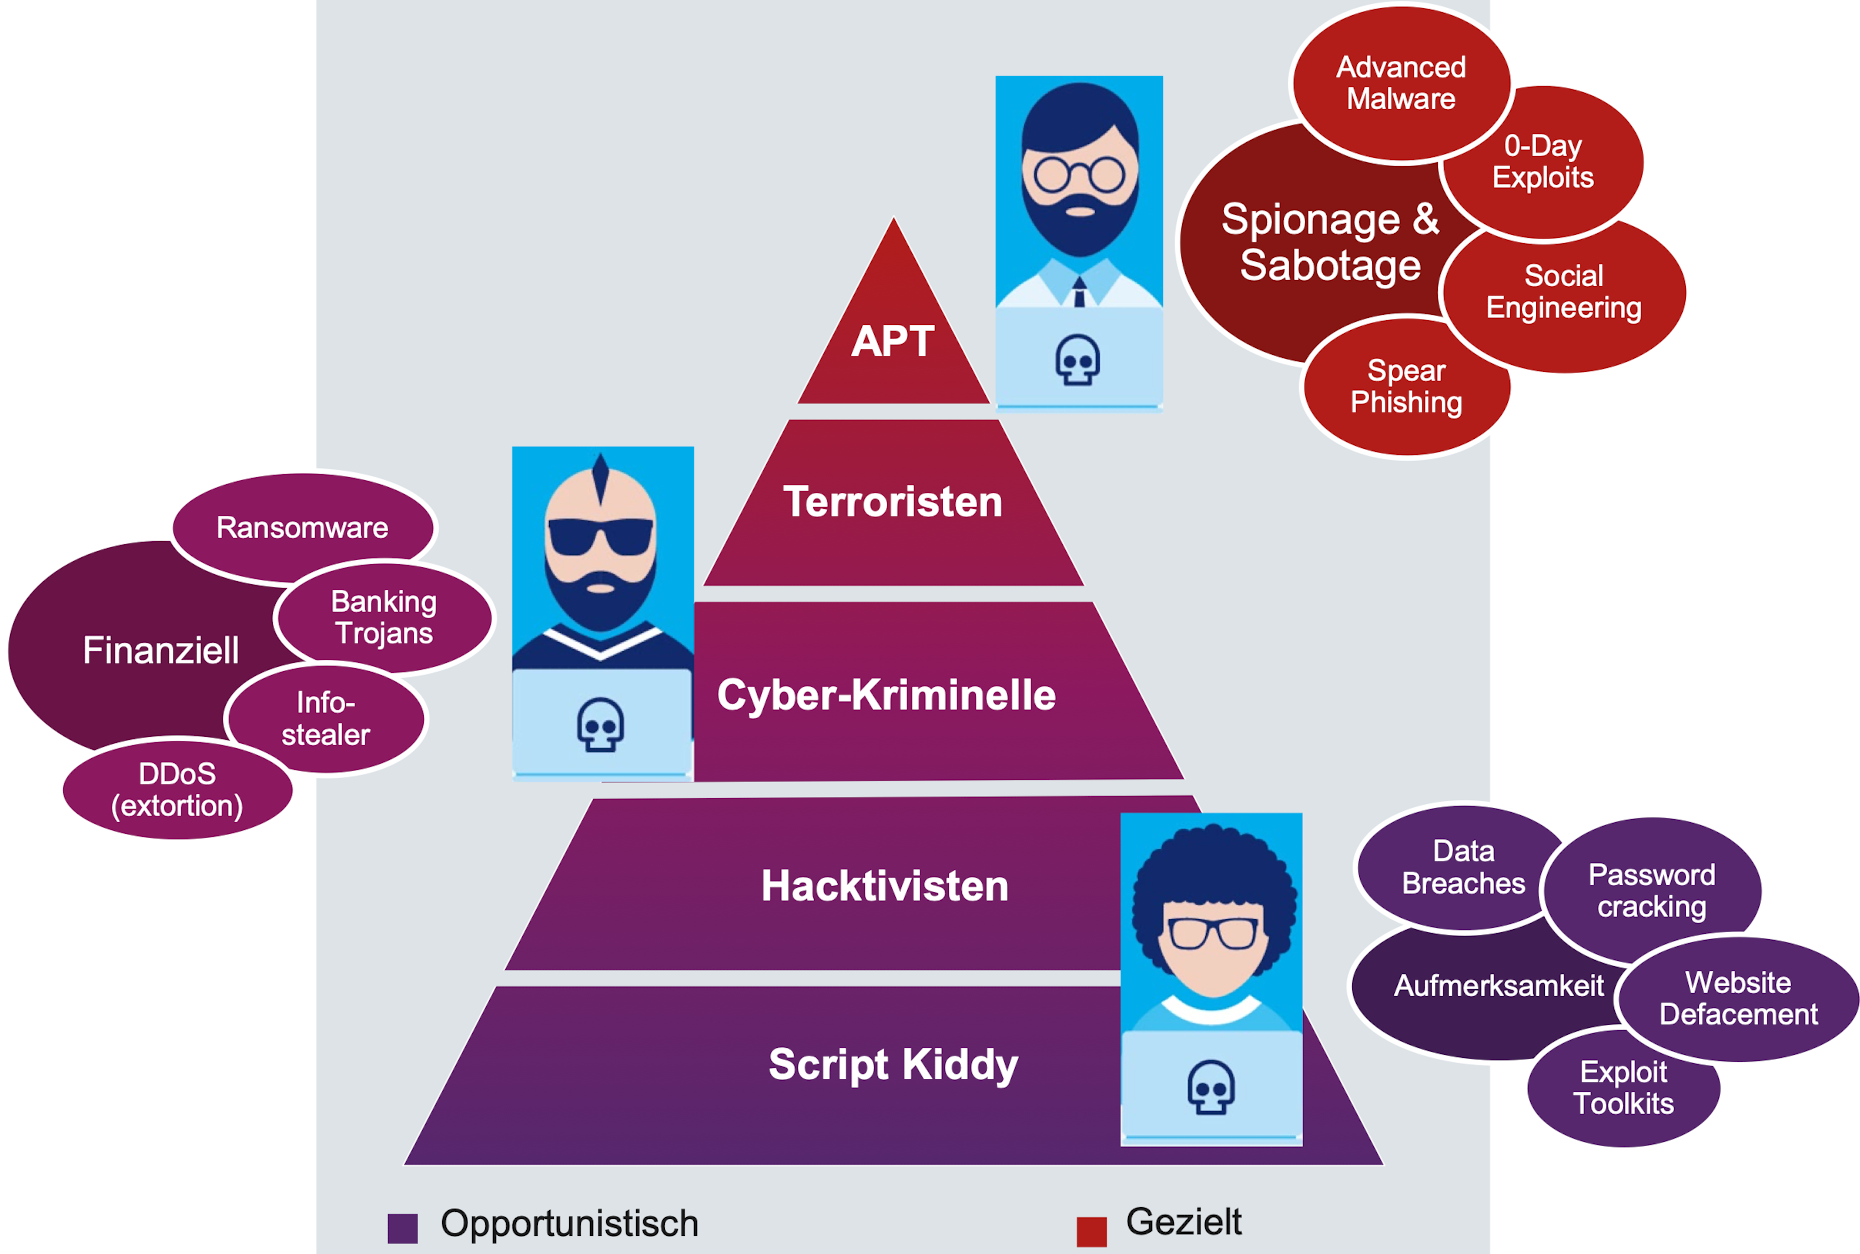
\includegraphics[width=.8\linewidth]{./img/01-cyber_defense/threat_actors}
    \vspace{-8pt}
\end{center}


\subsubsection{Script Kiddy}
\vspace{-8pt}
\begin{multicols*}{2}
    \textbf{Motivation}
    \begin{itemize}
        \item Aufmerksamkeit
        \item Anerkennung unter Ihresgleichen
        \item Opportunistisch
    \end{itemize}
    \columnbreak
    \textbf{Fähigkeiten}
    \begin{itemize}
        \item Wenige Fähigkeiten und Kenntnisse
        \item Nutzen verfügbare Hacking Tools
    \end{itemize}
\end{multicols*}
\vspace{-8pt}


\subsubsection{Hacktivisten}
\vspace{-8pt}
\begin{multicols*}{2}
    \textbf{Motivation}
    \begin{itemize}
        \item Aufmerksamkeit
        \item Anerkennung unter Gleichgesinnten
        \item Protest zum Ausdruck bringen
        \item Gezielt
    \end{itemize}
    \columnbreak
    \textbf{Fähigkeiten}
    \begin{itemize}
        \item Variieren sehr stark
        \item Wenig bis sehr Fortgeschritten
    \end{itemize}
\end{multicols*}
\vspace{-8pt}


\subsubsection{Übersicht: Script Kiddy \& Hacktivisten}
\begin{minipage}{0.3\linewidth}
    \begin{itemize}
        \item \textbf{P0:}\\ Erster eingenommener Server
        \item \textbf{TD:}\\ Ziel des Angreifers
    \end{itemize}
    \vfill
    $ $
\end{minipage}
\begin{minipage}{0.7\linewidth}
    \begin{center}
        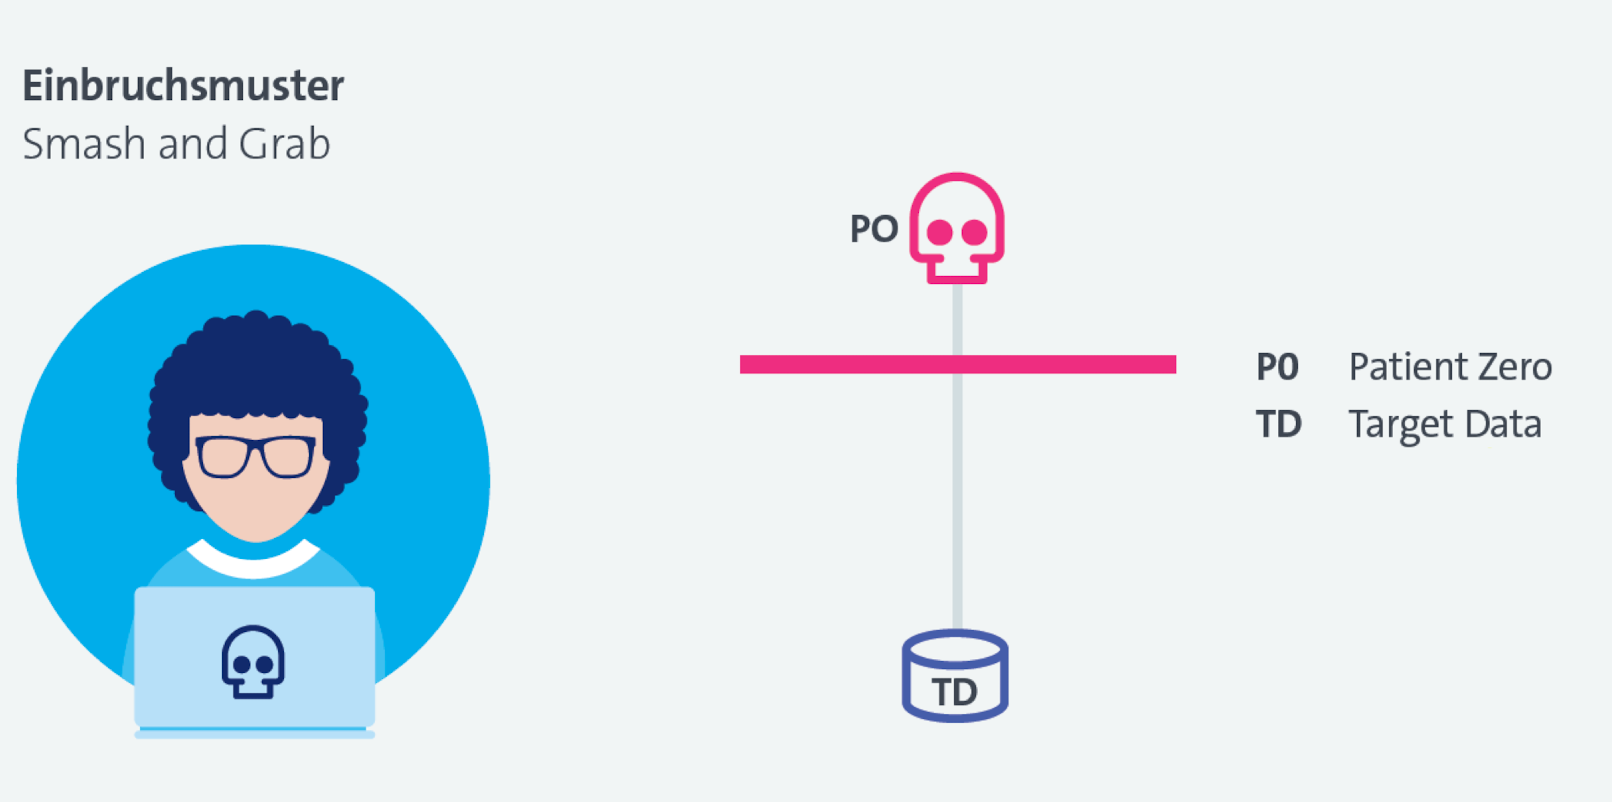
\includegraphics[width=\linewidth]{./img/01-cyber_defense/script_hacktivist}
    \end{center}
\end{minipage}

\textbf{Script Kiddys} und \textbf{Hacktivisten} zielen primär auf direkt exponierte Systeme ab wie beispielsweise Webserver. Sie zeichnen sich dadurch aus, dass sie schnellstmöglich ihren «Smash and Grab-Erfolg» bekannt geben wollen. Sie dringen in den wenigsten Fällen über längere Zeit in Netzwerke ein.


\subsubsection{Cyber-Kriminelle}
\vspace{-8pt}
\begin{multicols*}{2}
    \textbf{Motivation}
    \begin{itemize}
        \item Finanzieller Art, erpressen sehr viel Geld oder stehlen wertvolle Daten
        \item Opportunistisch
    \end{itemize}
    \columnbreak
    \textbf{Fähigkeiten}
    \begin{itemize}
        \item Hohe Professionalisierung
        \item Insider bieten in Untergrundforen an
        \item Setzen Angriffsmittel gegen eine breite Palette von Zielen ein
    \end{itemize}
\end{multicols*}


\vfill
$ $
\columnbreak


\subsubsection{Terroristen}
\vspace{-8pt}
\begin{multicols*}{2}
    \textbf{Motivation}
    \begin{itemize}
        \item Sabotage, Schaden \& Chaos anrichten
        \item Angst verbreiten
        \item Aufmerksamkeit und Rekrutierung
    \end{itemize}
    \vfill
    \columnbreak
    \textbf{Fähigkeiten}
    \begin{itemize}
        \item Angriffe auf kritische Systeme befürchtet, aber noch keine bekannt
        \item Nicht-staatliche, terroristische Gruppen scheinen Fähigkeit für gezielte Cyber-Angriffe noch nicht aufgebaut zu haben
    \end{itemize}
\end{multicols*}
\vspace{-8pt}


\subsubsection{Übersicht: Cyber-Kriminelle \& Terroristen}
\begin{minipage}{0.3\linewidth}
    \begin{itemize}
        \item \textbf{P0:}\\ Erster eingenommener Server
        \item \textbf{TD:}\\ Ziel des Angreifers
        \item \textbf{LM:}\\ Bewegung im\\ Netzwerk
        \item \textbf{P:}\\ Hintertüre
    \end{itemize}
    \vfill
    $ $
\end{minipage}
\begin{minipage}{0.7\linewidth}
    \begin{center}
        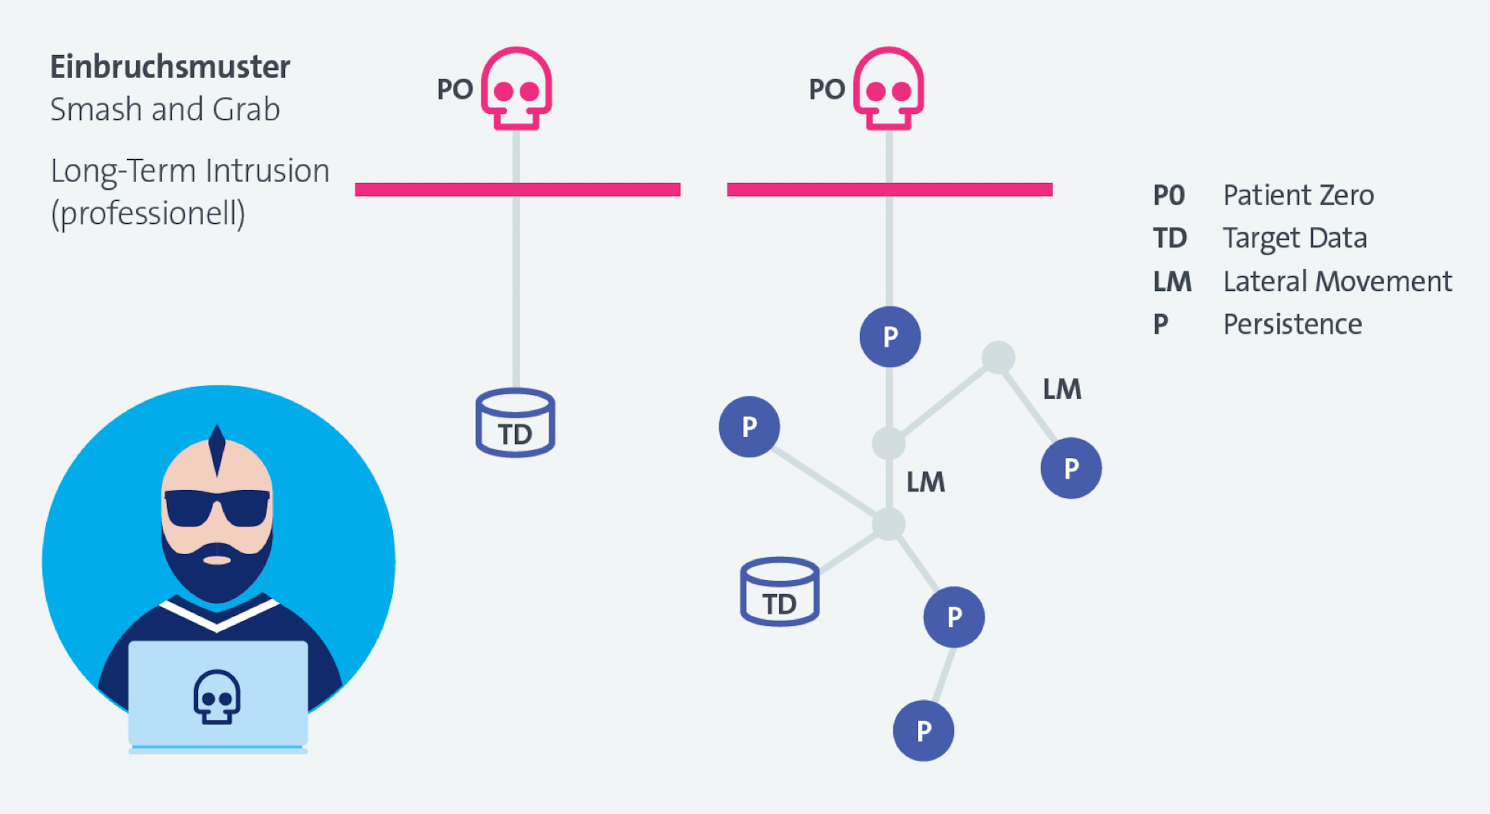
\includegraphics[width=\linewidth]{./img/01-cyber_defense/cyber_terrorists}
    \end{center}
\end{minipage}

\textbf{Cyber-Kriminelle} benötigen eine erheblich lange Verweildauer in den Systemen, um an die gewünschten Daten zu kommen und stehen oftmals in ihren technischen Fähigkeiten vielen APTs in nichts nach. Der entscheidende
Unterschied liegt jedoch in den strategischen Zielen.


\subsubsection{Advanced Persistent Threat (APT)}
\vspace{-8pt}
\begin{multicols*}{2}
    \textbf{Motivation}
    \begin{itemize}
        \item Klare Mission
        \item meist staatliche Ziele
        \item Spionage, politisch/ militärisch
        \item Sabotage, Schaden anrichten
        \item Sehr gezielt
    \end{itemize}
    \vfill
    \columnbreak
    \textbf{Fähigkeiten}
    \begin{itemize}
        \item Königsklasse
        \item staatlich / staatlich-finanziert
        \item ,,low-and-slow``, bleiben lange unbemerkt im Netzwerk und dringen erneut ein
        \item Nutzen eigene Tools, wie auch allgemein verfügbare ,,off-the-shelf`` Hacking Tools und Exploits
        \item Kombinieren mehrere Angriffsmethoden und -techniken
        \item Von Menschen koordinierte Aktionen
    \end{itemize}
\end{multicols*}
\vspace{-8pt}

\begin{minipage}{0.3\linewidth}
    \begin{itemize}
        \item \textbf{P0:}\\ Erster eingenommener Server
        \item \textbf{TD:}\\ Ziel des Angreifers
        \item \textbf{LM:}\\ Bewegung im\\ Netzwerk
        \item \textbf{P:}\\ Hintertüre
    \end{itemize}
    \vfill
    $ $
\end{minipage}
\begin{minipage}{0.7\linewidth}
    \begin{center}
        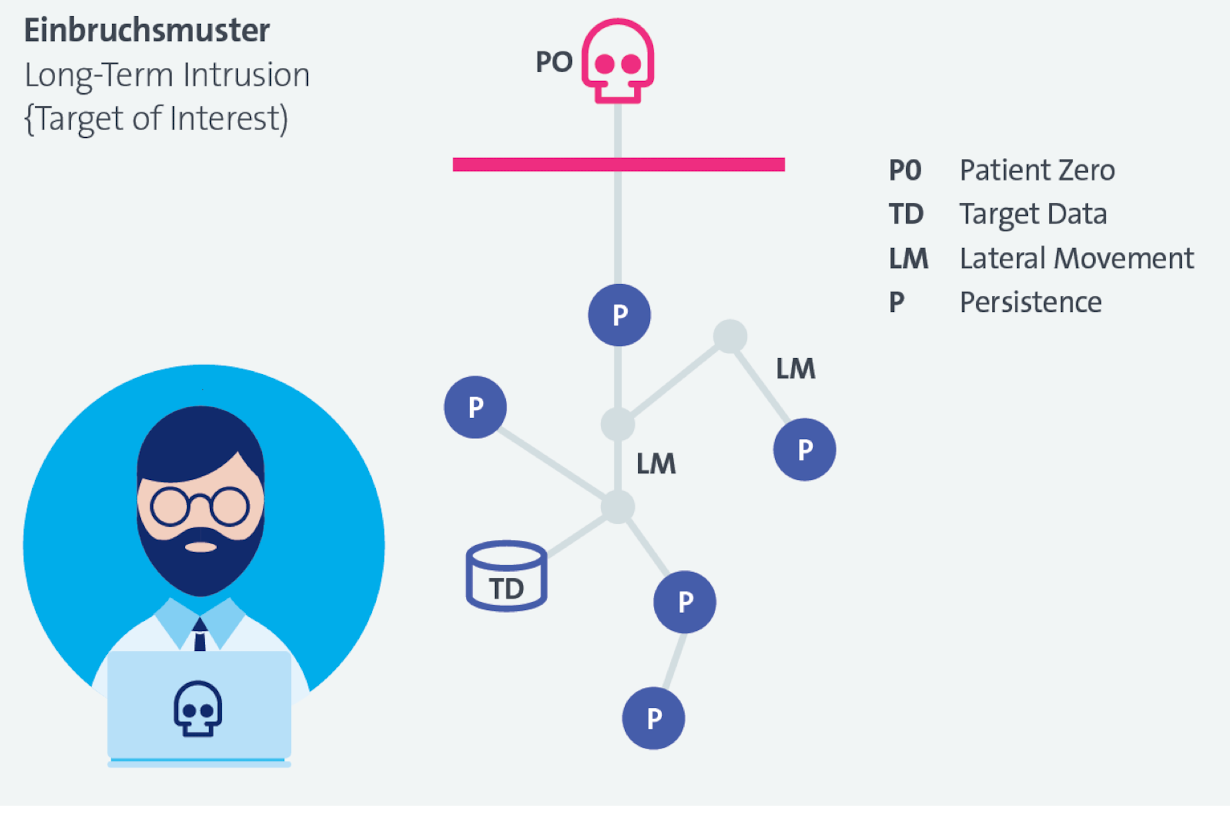
\includegraphics[width=\linewidth]{./img/01-cyber_defense/apt}
    \end{center}
\end{minipage}


\textbf{APTs} verbleiben in den meisten Fällen \textbf{sehr lange im Netzwerk} des Opfers (in der Regel mehr als 200 Tage) und betreiben einen entsprechend hohen Aufwand, um ihren Zugang über mehrere Wege sicherzustellen.
\textbf{Deshalb sollte das gesamte Ausmass des Angriffs unbedingt erst verstanden sein bevor man einen APT Angriff stoppt.}


\subsubsection{APT erklärt}
\textbf{Ablauf eines Angriffes:}
\begin{enumerate}
    \item Initial Infection: Ein Client wird infiziert.
    \item Es gibt noch keine Sicherheitslücke
    \item Client kommuniziert mit Command \& Control Server über längere Zeit
    \item Sobald ein Exploit bekannt ist, wird dieser ausgenutzt, bevor neuer Patch installiert wird
\end{enumerate}

\begin{center}
    \vspace{-8pt}
    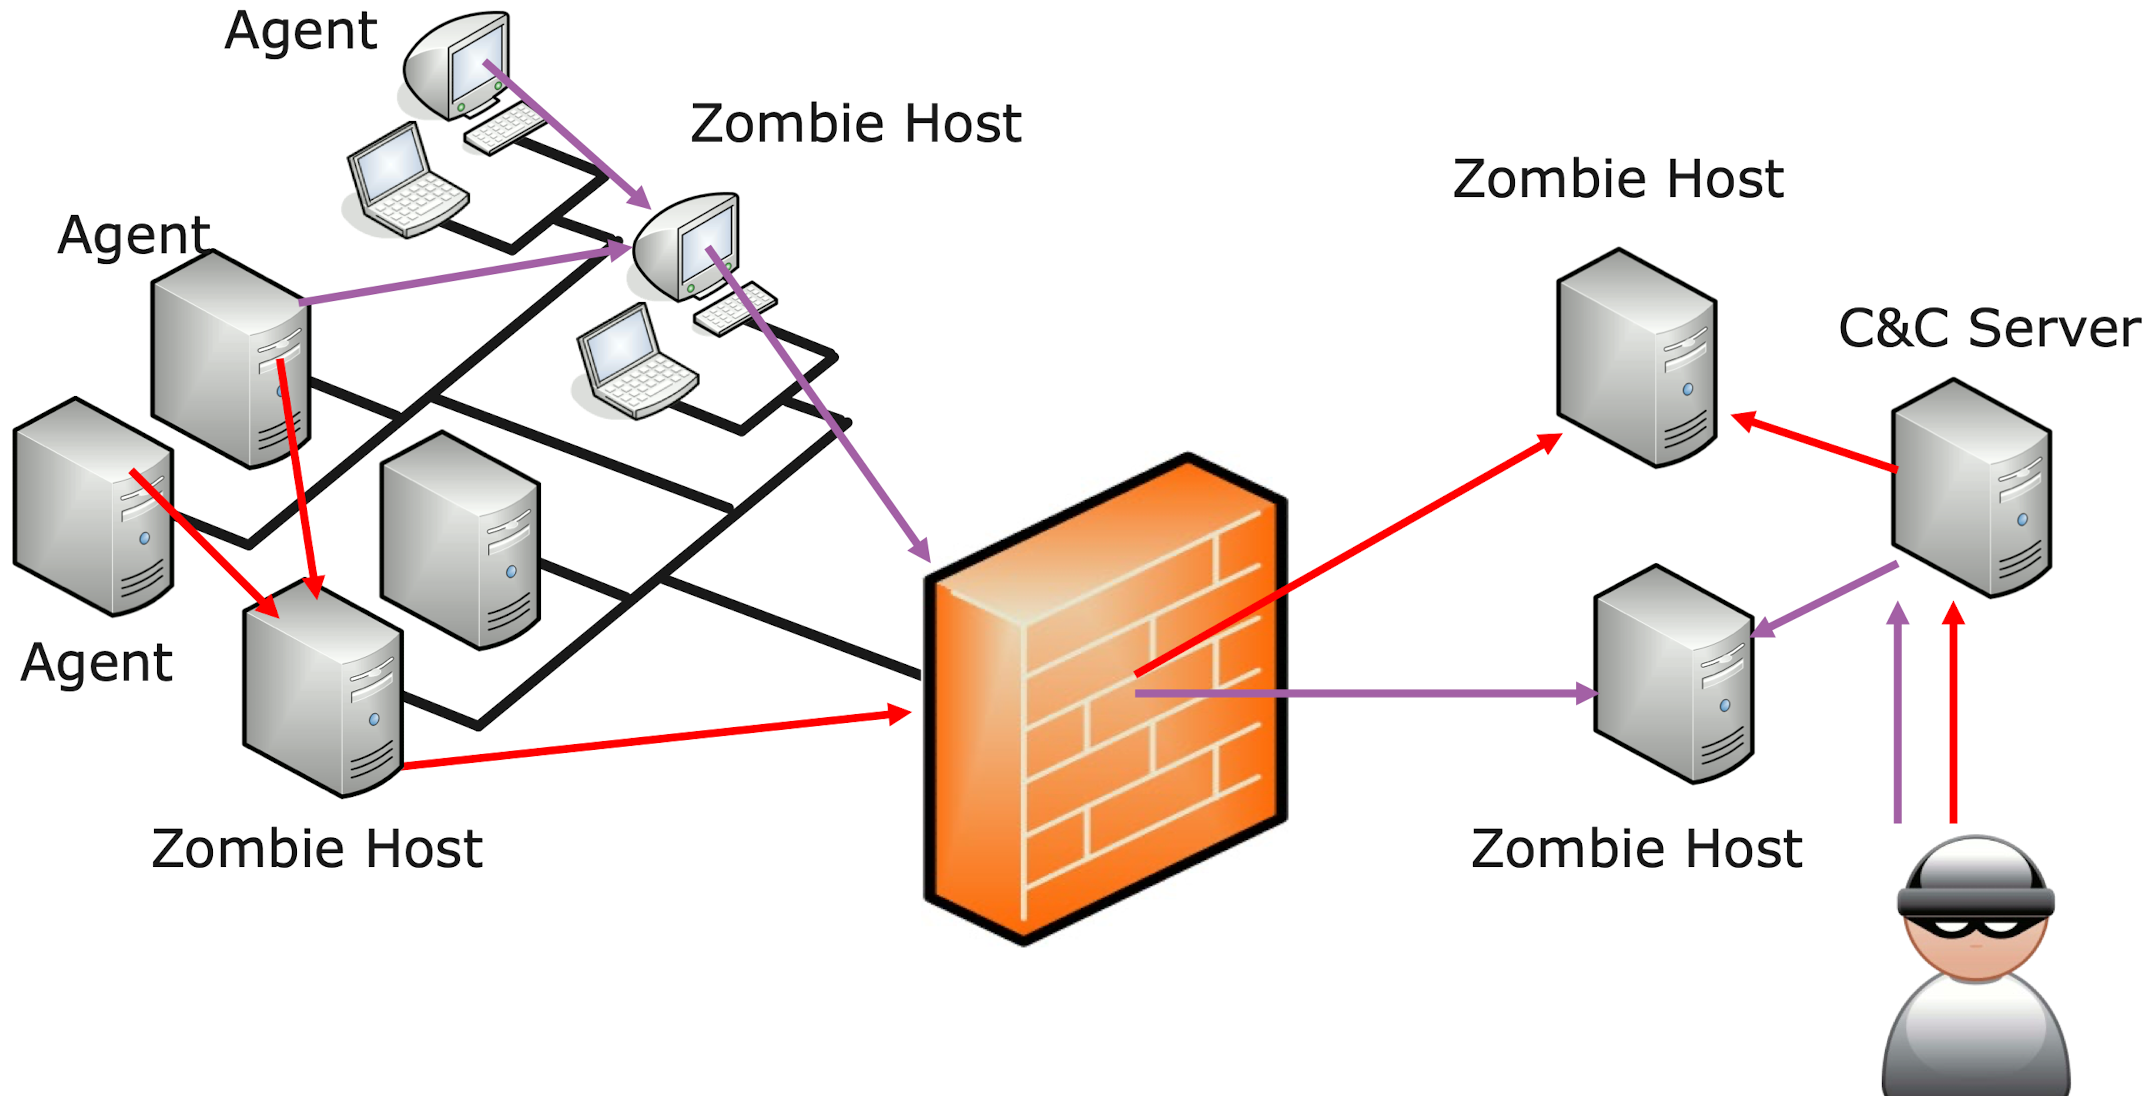
\includegraphics[width=.8\linewidth]{./img/01-cyber_defense/apt_diagram}
    \vspace{-8pt}
\end{center}

\begin{center}
    \vspace{-8pt}
    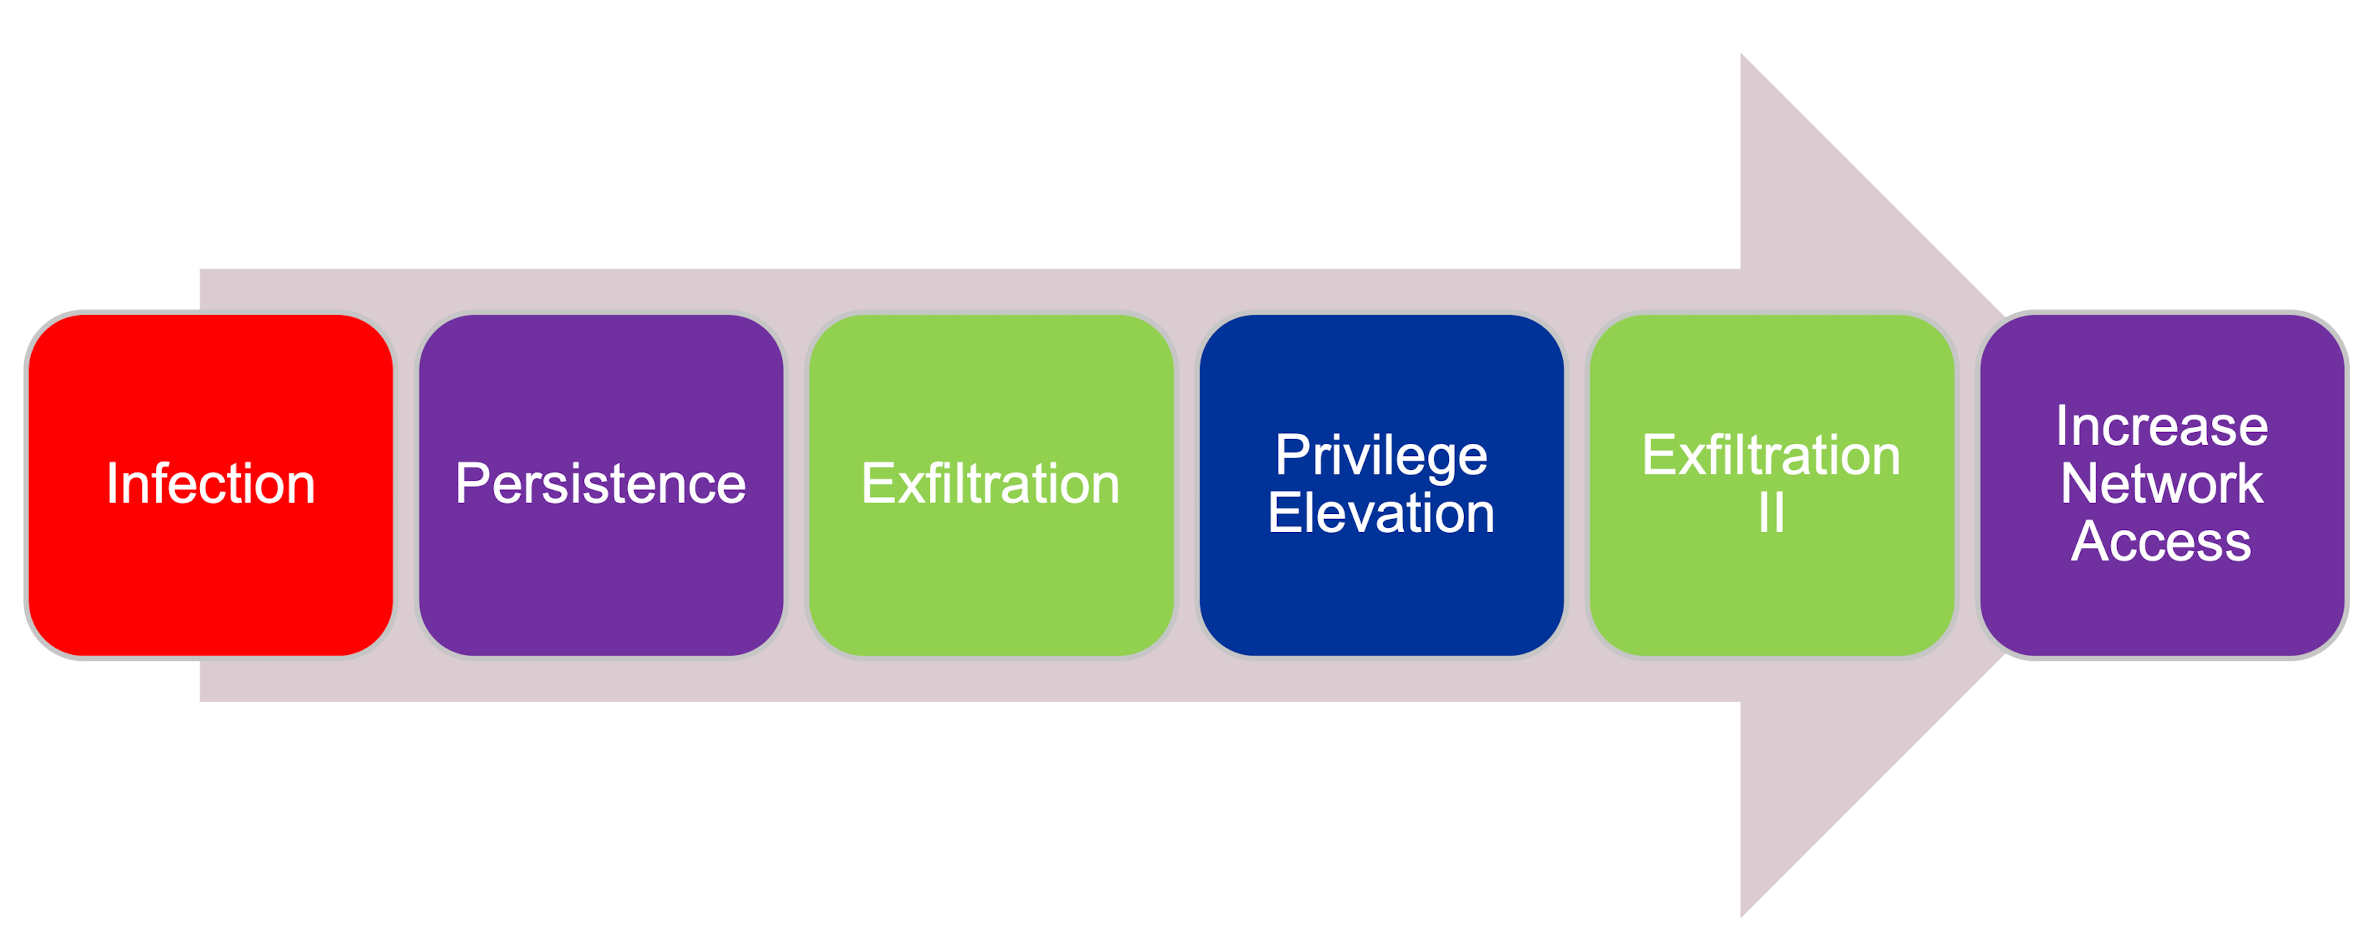
\includegraphics[width=.8\linewidth]{./img/01-cyber_defense/apt_process}
    \vspace{-8pt}
\end{center}

\subsection{Methoden der Hacker}\label{subsec:methoden-der-hacker}

\subsubsection{Direct Attack}
\begin{itemize}
    \item Brute-Force-Angriff
    \item Angriff auf offene FW Ports
\end{itemize}


\subsubsection{Indirect Attack}
\begin{itemize}
    \item Virus
    \item Malware
    \item Ransomware
\end{itemize}


\subsubsection{Man-in-the-Middle Attack}
Mehr Informationen hier: \nameref{subsubsec:man-in-the-middle}
\begin{itemize}
    \item Im Netzwerk dazwischen schalten
\end{itemize}


\subsubsection{Man-in-the-Browser}
Mehr Informationen hier: \nameref{subsubsec:man-in-the-browser}
\begin{itemize}
    \item Direkt im Browser dazwischenschalten
    \item gain root, gain Administrator
\end{itemize}


\subsubsection{Privilege Elevation}
\begin{itemize}
    \item Rechte erhöhen, um diese auszunutzen
\end{itemize}


\subsubsection{APT and Data Exfiltration}
\begin{itemize}
    \item Komplexer Angriff
    \item Command and Control Server
    \item Zombie Host, welcher mit C\&C kommuniziert
\end{itemize}

\subsubsection{Social Engineering}
\begin{itemize}
    \item Identitätsdiebstahl
\end{itemize}

\subsubsection{MITRE}
\begin{itemize}
    \item MITRE ATT\&CK Framework
\end{itemize}

\vfill
$ $
